This manuscript
(\href{https://georgiadoing.github.io/paper_test/v/e0430d5da4de899c144861e386b7ec516d456c0a/}{permalink})
was automatically generated
from \href{https://github.com/georgiadoing/paper_test/tree/e0430d5da4de899c144861e386b7ec516d456c0a}{georgiadoing/paper\_test@e0430d5}
on July 1, 2025.

\hypertarget{authors}{%
\subsection{Authors}\label{authors}}

\begin{itemize}
\item
  \textbf{Georgia Doing}
  
\includegraphics[width=0.16667in,height=0.16667in]{images/orcid.svg}
  \href{https://orcid.org/0000-0002-0835-6955}{0000-0002-0835-6955}
  · 
\includegraphics[width=0.16667in,height=0.16667in]{images/github.svg}
  \href{https://github.com/georgiadoing}{georgiadoing}
  Department of Dermatology, Duke Univeristy
  · Funded by Grant F32XXXXX, LRPXXXXX
\item
  \textbf{Julia Oh}
  \textsuperscript{\protect\hyperlink{correspondence}{✉}}
  · 
\includegraphics[width=0.16667in,height=0.16667in]{images/github.svg}
  \href{https://github.com/janeroe}{janeroe}
  Department of Dermatology, Duke Univeristy; Microbiome Center, Duke Univeristy
  · Funded by Grant RO1XXX
\end{itemize}

\leavevmode\vadjust pre{\hypertarget{correspondence}{}}%
✉ --- Correspondence possible via \href{https://github.com/georgiadoing/paper_test/issues}{GitHub Issues}
or email to
Julia Oh \textless julia.oh@duke.edu\textgreater.

\hypertarget{abstract}{%
\subsection{Abstract}\label{abstract}}

Background Of the trillions of microbial cells associated with human skin, less than half are identifiable at or below the species level, a quarter are culturable, and only a handful have been isolated for extensive laboratory study. Both species and strain-level genetic diversity are increasingly appreciated as important for microbial community function in healthy and diseases states of the skin. However, while sequencing technologies readily unveil genetic diversity in the skin microbiome, the overwhelming numbers of species, strains, and genes with unknown function limit our ability to interpret available data.

Methods: We have developed a method for the re-analysis of public transcriptomic datasets from multiple strains of \emph{S. aureus} and \emph{S. epidermidis} and the generation of hypotheses for gene functions using unsupervised transfer learning neural networks for data compression and latent feature representation. Further, we have tested consequences of gene knock-down using targeted and genome-wide CRISPR-interference screening as validation of our hypothesis generation methods.

Results:, Using our novel methods we have hypothesized roles for yet uncharacterized conserved and species-specific genes in \emph{S. epidermidis} stress responses including growth under metal depletion and oxidative stress. CRISPRi-interference screening suggests genes identified by our pipeline contribute to growth under these respective stress conditions.

Discussion: These methods for identifying microbial gene function are important because they wrangle microbial genetic and transcriptomic diversity to identify novel therapeutic targets and modulators of virulence on the skin.

\hypertarget{introduction}{%
\subsection{Introduction}\label{introduction}}

Testing a citation {[}\protect\hyperlink{ref-754TZ3KR}{1}{]} and {[}\protect\hyperlink{ref-f98SpRHX}{2}{]}.

Also testing tables

\begin{longtable}[]{@{}lll@{}}
\caption{Caption for this example table. \label{tbl:example-id}}\label{tbl:example-id}\tabularnewline
\toprule()
Column 1 & Column 2 & Column 3 \\
\midrule()
\endfirsthead
\toprule()
Column 1 & Column 2 & Column 3 \\
\midrule()
\endhead
value\_a & 1 & 47 \\
value\_b & 2 & 56 \\
\bottomrule()
\end{longtable}

And lastly, figures

\begin{fignos:no-prefix-figure-caption}

\begin{figure}
\centering
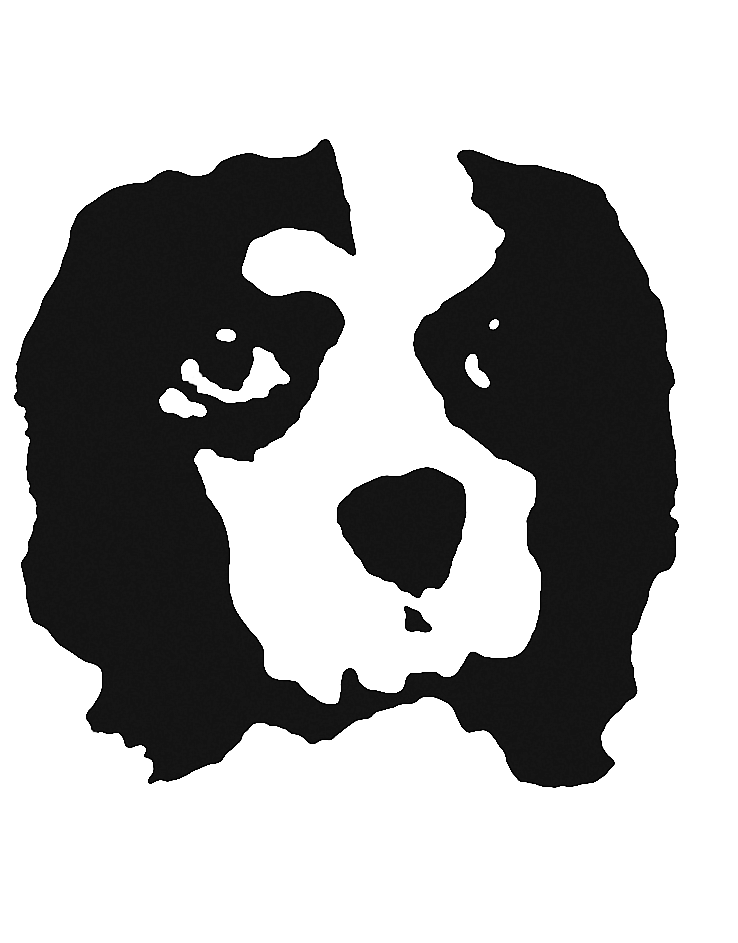
\includegraphics{images/ginny_stamp_pic.png}
\caption{Ginny stamp}
\end{figure}

\end{fignos:no-prefix-figure-caption}

\hypertarget{references}{%
\subsection{References}\label{references}}

\hypertarget{refs}{}
\begin{CSLReferences}{0}{0}
\leavevmode\vadjust pre{\hypertarget{ref-754TZ3KR}{}}%
\CSLLeftMargin{1. }%
\CSLRightInline{\textbf{SkinCom, a synthetic skin microbial community, enables reproducible investigations of the human skin microbiome}
\CSLBlock{Asama Lekbua, Deepan Thiruppathy, Joanna Coker, Yuhan Weng, Fatemeh Askarian, Armin Kousha, Clarisse Marotz, Amber Hauw, Victor Nizet, Karsten Zengler} \emph{Cell Reports Methods} (2024-08) \url{https://doi.org/g9rx6g}
\CSLBlock{DOI: \href{https://doi.org/10.1016/j.crmeth.2024.100832}{10.1016/j.crmeth.2024.100832} · PMID: \href{https://www.ncbi.nlm.nih.gov/pubmed/39111313}{39111313} · PMCID: \href{https://www.ncbi.nlm.nih.gov/pmc/articles/PMC11384088}{PMC11384088}}}

\leavevmode\vadjust pre{\hypertarget{ref-f98SpRHX}{}}%
\CSLLeftMargin{2. }%
\CSLRightInline{\textbf{Skin-associated \textless i\textgreater Corynebacterium amycolatum\textless/i\textgreater{} shares cobamides}
\CSLBlock{MH Swaney, N Henriquez, T Campbell, J Handelsman, LR Kalan} \emph{mSphere} (2025-01-28) \url{https://www.ncbi.nlm.nih.gov/pmc/articles/PMC11774034/}
\CSLBlock{DOI: \href{https://doi.org/10.1128/msphere.00606-24}{10.1128/msphere.00606-24} · PMID: \href{https://www.ncbi.nlm.nih.gov/pubmed/39692507}{39692507} · PMCID: \href{https://www.ncbi.nlm.nih.gov/pmc/articles/PMC11774034}{PMC11774034}}}

\end{CSLReferences}
